
\documentclass[10pt,a4paper]{article}
\usepackage[utf8]{inputenc}
\usepackage[spanish]{babel}
\usepackage{amsmath}
\usepackage{amsfonts}
\usepackage{amssymb}
\usepackage{makeidx}
\usepackage{graphicx}
\usepackage{cite} % para contraer referencias
\usepackage{fourier}
\usepackage{xcolor}
\usepackage{hyperref}
 \usepackage{float}
\usepackage[bottom]{footmisc}
\usepackage[left=2cm,right=2cm,top=2cm,bottom=2cm]{geometry}
\title{Plan - sesión 6}


\author{\textbf{Victor M. Santos}\thanks{victorhugo\_m09@hotmail.com}, \textbf{M.Tarazona-Alvarado}\thanks{miguelta281@gmail.com}, \textbf{J. Pisco-Guabave} \thanks{jhojavi@gmail.com}. \\ Grupo Halley , \\ Universidad Industrial de Santander, Bucaramanga, Colombia.}


\date{ }


\begin{document}

\maketitle
\tableofcontents
\section{Objetivo}


\section{Contenido}
\begin{itemize}
\item Coordenadas geográficas
\item Coordenadas celestes
\begin{itemize}
\item Horizontales 
\item Ecuatoriales
\begin{itemize}
\item Horarias
\item Absolutas
\end{itemize}
\item Eclípticas 
\end{itemize} 
\end{itemize}


\section{Recursos}
\begin{itemize}
 \item Salón con capacidad para 20 personas
 \item Proyector
 \item Computador
 \item Marcadores
 \item Tablero
 \item Espacio al aire libre (amplio)
\end{itemize}

\section{Marco conceptual}
Las coordenadas son sistemas de referencia que aclaran la situación de un objeto para permitir su análisis. Por ejemplo: en astronomía, las coordenadas son esenciales para determinar la posición aparente de un objeto en la bóveda celeste. \\

\subsection{Coordenadas geográficas}
Estas coordenadas son trazadas sobre el globo terráqueo y las componen los meridianos y paralelos. Las líneas meridianas son trazadas de polo a polo e indican la latitud. En cambio, los paralelos son trazados de forma paralela con respecto al Ecuador; indican la longitud.
La latitud es el número correspondiente del paralelo y se cuenta en grados, minutos y segundos, y puede ser Norte o Sur. A su vez, la longitud es la distancia en grados, minutos y segundos desde el meridiano de Greenwich (de 0° a 180°), y puede ser longitud Este u Oeste.

\begin{figure}[H]
\centering
%\raggedright
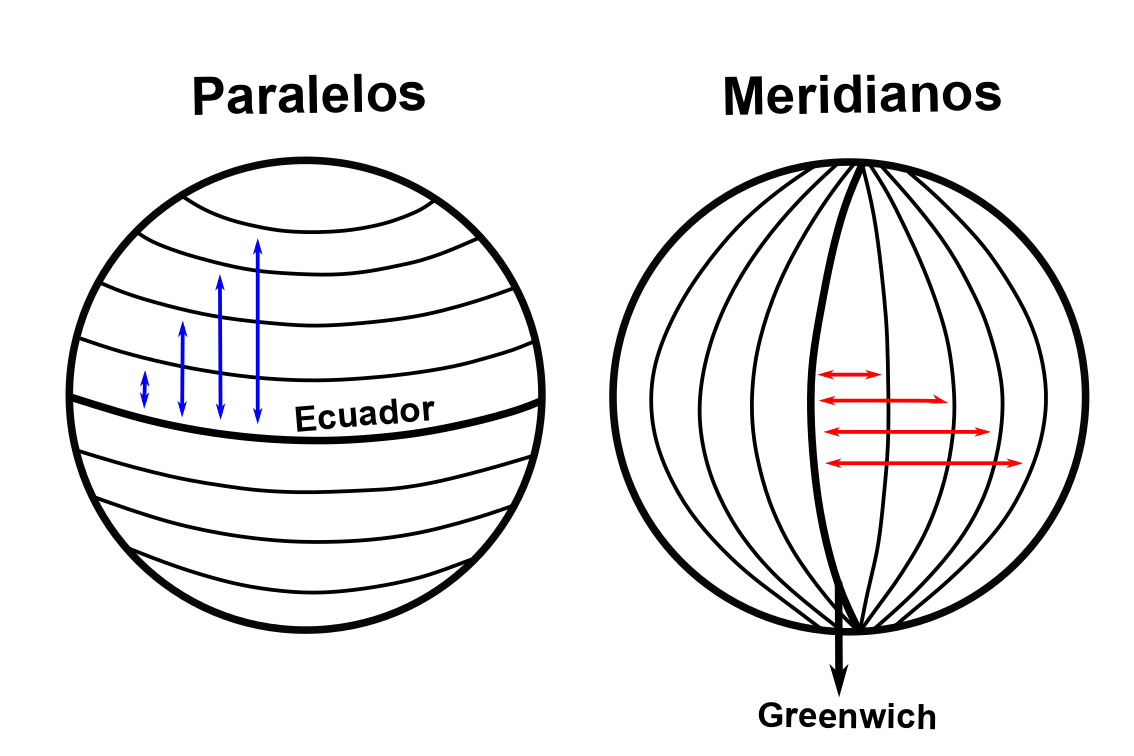
\includegraphics[scale=0.3]{Imagenes/Geograficas_01}
\end{figure}

\subsection{Coordenadas celestes}
Las coordenadas celestes permiten localizar la posición de los astros en la bóveda celeste. Para esto, se basan en el uso de ciertos ángulos determinados por un plano fundamental que sirve como referencia. En ese sentido, cada plano fundamental está ligado a un sistema coordenado diferente (ángulos diferentes).

\subsubsection{Coordenadas horizontales}
Las coordenadas horizontales (también conocidas como azimutales) son locales y su plano fundamental es el horizonte del observador. Particularmente, estas coordenadas funcionan con dos ángulos: el Azimut (o Acimut) y la Altura. El Acimut es un ángulo comprendido entre 0° y 360° medido sobre el plano horizontal del observador en dirección horaria e iniciando en el Sur (sin embargo, en algunas aplicaciones y wikipedia :v se toma como punto inicial el Norte). Por otro lado, la Altura es el ángulo medido sobre el círculo vertical que pasa por la posición del astro y va desde 0° a 90° o de 0° a -90°.

\begin{figure}[H]
\centering
%\raggedright
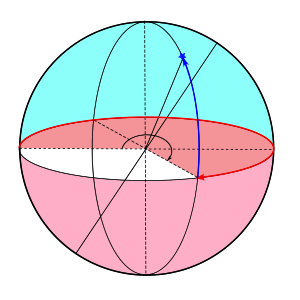
\includegraphics[scale=0.3]{Imagenes/C_horizontales_01}
\end{figure}


\subsubsection{Coordenadas ecuatoriales horarias}
Las coordenadas ecuatoriales horarias tienen como plano fundamental el Ecuador Celeste. Los ángulos claves para estas coordenadas son: el Ángulo Horario y la Declinación. El Ángulo Horario se forma entre el meridiano que pasa por el lugar y el meridiano del astro observado, iniciando su medición desde el meridiano local hacia el Oeste. Es usual que este ángulo sea representado en unidades temporales, pues representa el tiempo transcurrido desde que el astro pasó por el meridiano local. En ese sentido, este ángulo puede ir de 0° a 360° comprenderse entre 0 horas y 24 horas. En cambio, la Declinación es el ángulo medido desde el Ecuador a lo largo del meridiano que pasa por el astro, este comprende valores de 0° a 90° y entre 0° y -90°.


\begin{figure}[H]
\centering
%\raggedright
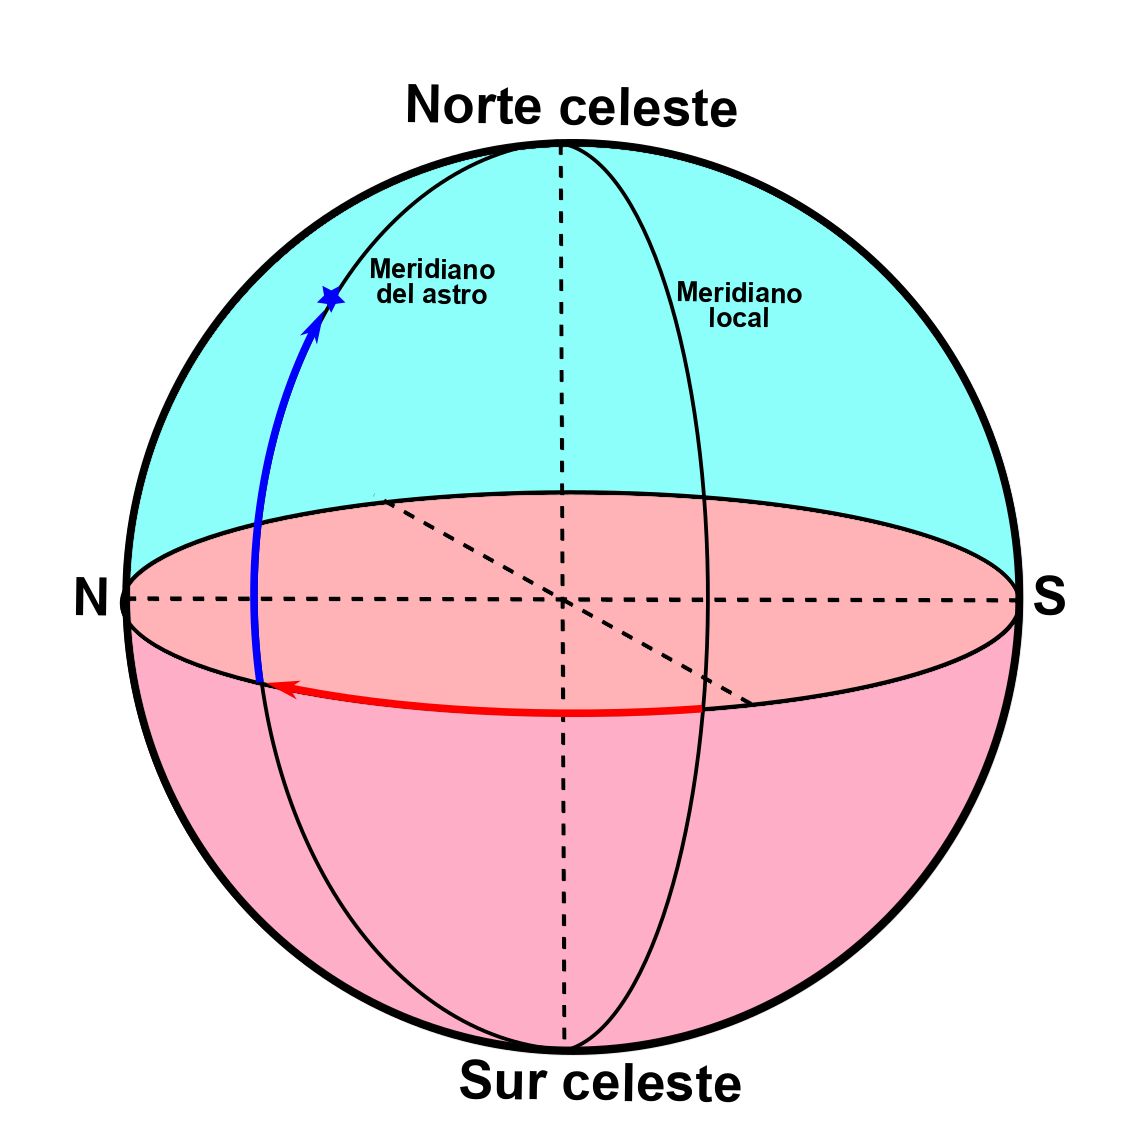
\includegraphics[scale=0.3]{Imagenes/C_Ecua_horarias_01}
\end{figure}

\subsubsection{Coordenadas ecuatoriales absolutas}
Las coordenadas ecuatoriales absolutas tienen como plano fundamental el Ecuador Celeste. Sus ángulos son conocidos como Ascensión Recta y Declinación. La Ascensión Recta es el ángulo medido sobre el Ecuador Celeste entre el punto Aries y el meridiano que pasa por el astro, se mide en dirección antihoraria y oscila entre valores de 0° a 360°. De forma semejante, la Declinación es el ángulo medido desde el Ecuador a lo largo del meridiano que pasa por el astro, comprende valores de 0° a 90° y entre 0° y -90°.

\begin{figure}[H]
\centering
%\raggedright
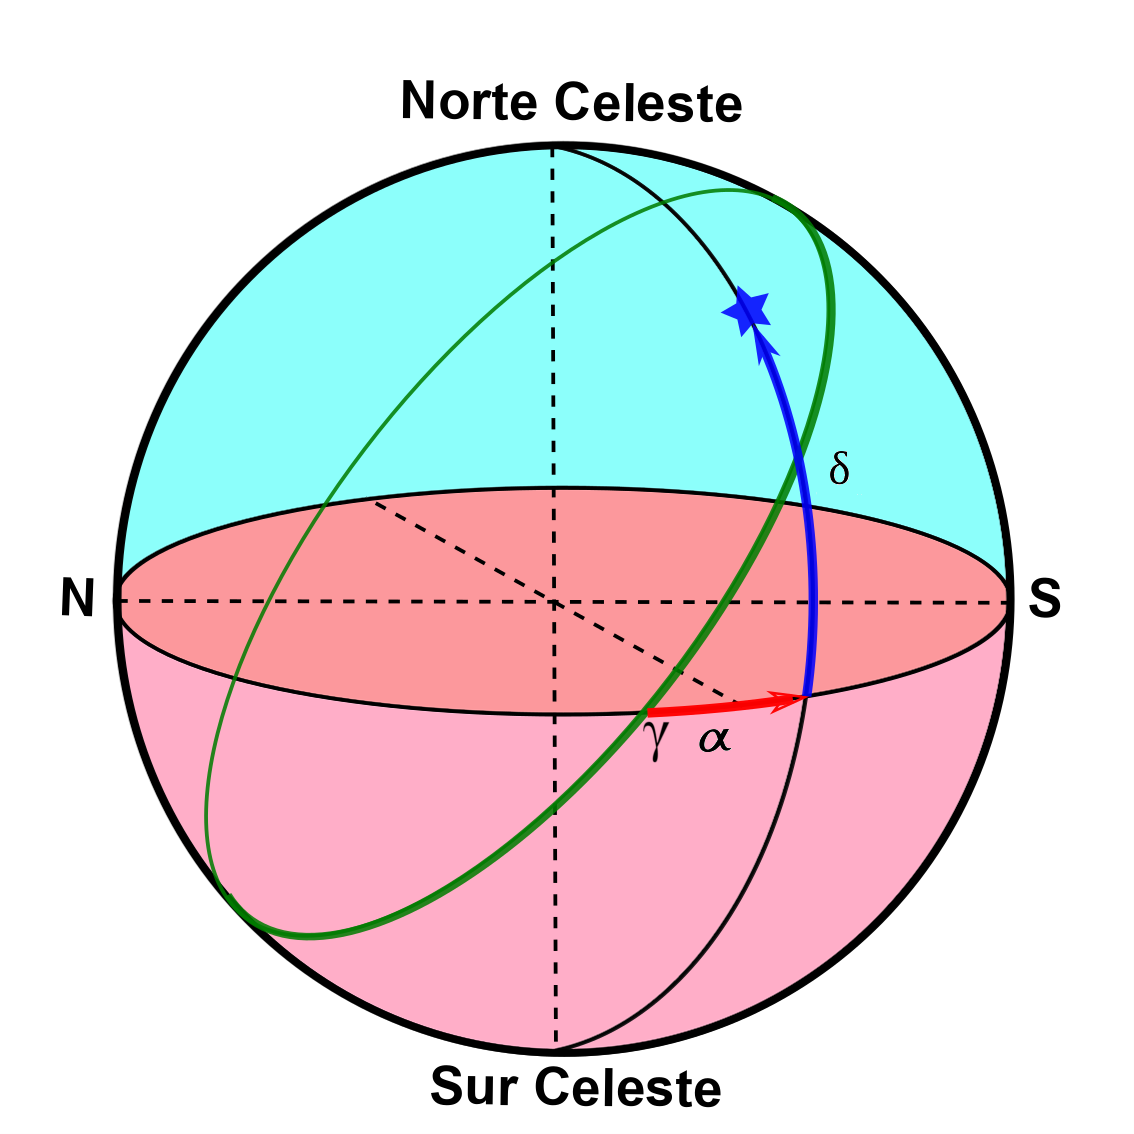
\includegraphics[scale=0.3]{Imagenes/C_Ecua_Abs_01}
\end{figure}

\subsubsection{Coordenadas eclípticas}
Las coordenadas eclípticas toman como plano fundamental la Eclíptica. Sus ángulos son la Longitud y la Latitud. La Longitud se mide sobre la Eclíptica y es descrito como el ángulo formado entre el punto Aries y el meridiano eclíptico que pasa por el astro, oscilando entre 0° y 360° en dirección horaria. En cuanto a la Latitud, es el ángulo medido a partir de la Eclíptica hacia el Norte o Sur eclípticos; los valores van de 0° a 90° N o de 0° a 90° S.

\begin{figure}[H]
\centering
%\raggedright
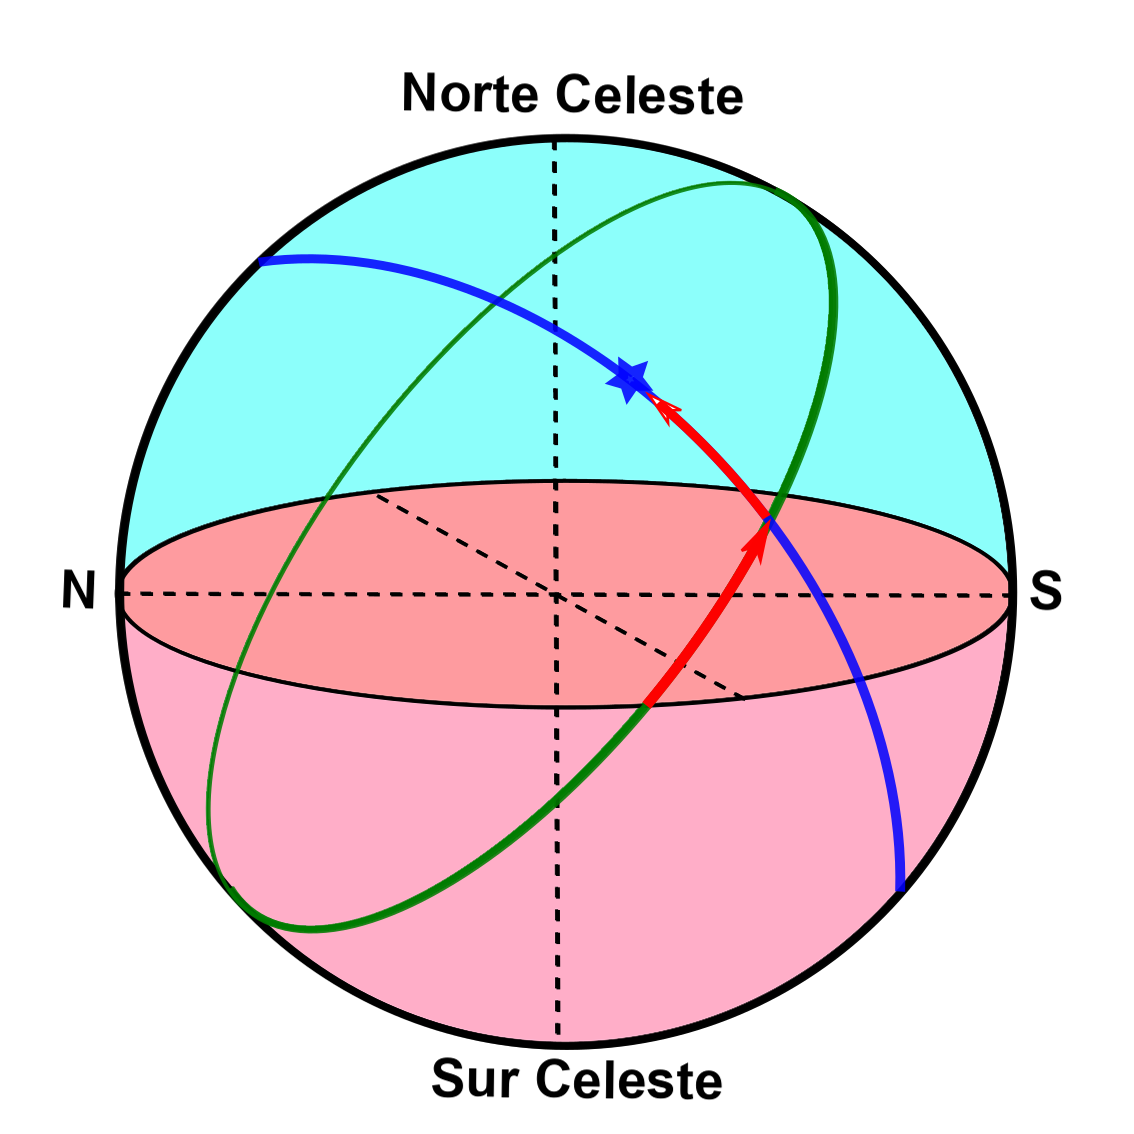
\includegraphics[scale=0.3]{Imagenes/C_Eclip_01}
\end{figure}

\section{Planeación de la sesión}
\begin{table}[H]
\begin{tabular}{|l|l|l|l|}
\hline
\textbf{Etapa}      & \textbf{Tiempo} & \textbf{Actividad}      & \textbf{Recursos}   \\ \hline
\textbf{Inicio}     & 20 minutos      & S05AI01      & \begin{tabular}[c]{@{}l@{}}- Computador \\ - Proyector  \end{tabular} \\ \hline
\textbf{Desarrollo} &   60 minutos  &  \begin{tabular}[c]{@{}l@{}}S05AD01  \\ S05AD02 \\ S05AD03 \\ S05AD04    \end{tabular}                                                                                       & \begin{tabular}[c]{@{}l@{}}- Prisma \\ - Globos \\ - Lupas \\ - Linterna (luz blanca) - Sextante \\ Cartulina (1/8)  \\ \end{tabular} \\ \hline
\textbf{Cierre}     &   40 minutos              &  S05AC01                                                                                    & \begin{tabular}[c]{@{}l@{}} - Tubo \\ - CD \\ - Cinta (negra) \\ - Cartulina \end{tabular} \\ \hline
\end{tabular}
\end{table}

\subsection{S06AI01}
Para esta actividad es necesario acceder al material de apoyo e imprimir la imagen que allí se encuentra. La actividad se hace en pares de estudiantes, siendo el ideal 10 grupos de 2 personas. El desarrollo de esta actividad consiste en ubicar 5 barcos sobre el mapamundi bajo las siguientes condiciones: 2 barcos están en tierra esperando a ser usados, y, 3 barcos están en diferentes zonas del mar. Luego, cada estudiante debe "atacar" a los barcos enemigos (de la pareja) dando las coordenadas en latitud y longitud.

\href{https://drive.google.com/open?id=12NxsFNSEWnwG91Cd1T0vwuFTxzpM6C9NfwtiAmDwlz8}{Material de apoyo}
\subsection{S06AD01}
En esta actividad se hará uso de dos instrumentos clásicos usados en astronomía: el cuadrante y el sextante marino u horizontal. Estos instrumentos permiten medir los ángulos relacionados con las Coordenadas Horizontales. En cuanto a la actividad a desarrollar, se dibujará en el suelo un círculo (preferiblemente con tiza) en el que los estudiantes tendrán que ubicar ciertos objetos claves que el tutor ubicó en diferentes posiciones con anterioridad. El estudiante debe de ubicar al menos 2 objetos indicando su posición en coordenadas horizontales, y, debe hacerlo con la mayor rapidez posible. Se recomienda al tutor otorgar un elemento de motivación a los estudiantes para incentivar la participación en la actividad.


\subsection{S06AD02}
Para esta actividad se usará la esfera armilar. Consiste en representar las Coordenadas Ecuatoriales en la esfera armilar. La labor del docente es la de explicar, usando la esfera como maqueta, el funcionamiento de las Coordenadas Ecuatoriales, tanto las Horarias como las Absolutas. Se recomienda que el uso de esta maqueta esté enfocado en diferenciar el ángulo horario, la ascensión recta y la declinación, abordando en paralelo las similitudes que estos ángulos presentan con los trabajados en Coordenadas Geográficas.

\subsection{S06AD03}
Presentación


\subsection{S06AC01}
\end{document}